\documentclass{article}
\usepackage[utf8]{inputenc}
\usepackage{float}
\usepackage{graphicx}
\graphicspath{{./images/}}

\title{Super Mario World AI}
\author{Siebren Cosijn}
\begin{document}
    \maketitle
    \section{Introduction}
    \begin{figure}[H]
    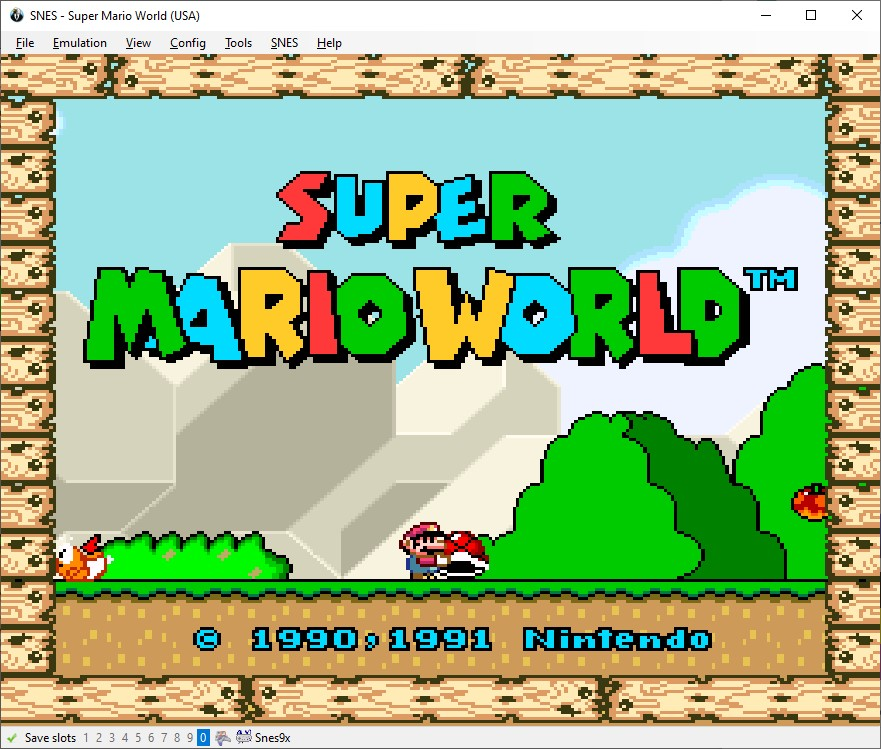
\includegraphics[width=.85\textwidth]{start-screen}
    \centering
    \end{figure}

    \section{Goals}

    \section{Preprocessing}
    \subsection{Discrete Actions}
    \begin{itemize}
        \item select, start, L, R not needed
        \item x and y same function
        \item movement: none, left, right, down, up
        \item jump: none, spin, jump
        \item special: none, special
        \item $5*3*2=30$ discrete actions
    \end{itemize}
    \begin{figure}[H]
    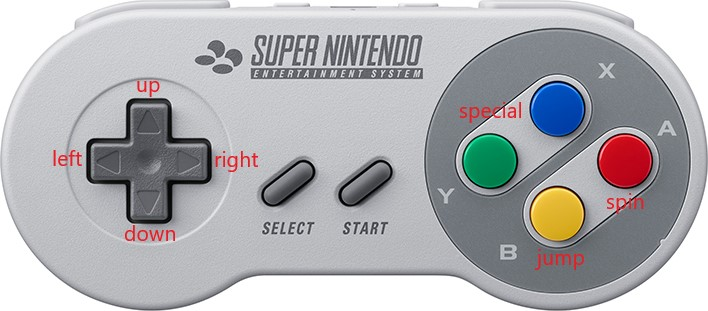
\includegraphics[width=.85\textwidth]{snes-controller-annot}
    \centering
    \end{figure}
    \subsection{Frame Manipulation}
    \subsubsection*{Skip frames}
    \begin{itemize}
        \item Consider every 4th frame
        \item Reduced training time
    \end{itemize}
    \subsubsection*{Resize frames}
    \begin{itemize}
        \item 84x84
        \item Grayscale
        \item Reduced memory requirement
    \end{itemize}
    \subsubsection*{Stack frames}

    \section{Model}

    \section{Training}

    \section{Results}
\end{document}